\documentclass[a4paper,12pt,french]{article}

\usepackage[cours]{../../Style}

%\selectcolormodel{cmyk}

%\usepackage{wrapfig}

% Début du document
%%%%%%%%%%%%%%%%%%%
\begin{document}

\title{Fonction dérivée}
\maketitle

\begin{programme}
\item Fonction dérivée
\item Dérivées de $x \mapsto x^2$, $x \mapsto x^3$, de combinaisons linéaires, de polynômes de degré $\leq 3$
\item Sens de variation d'une fonction, lien avec le signe de la dérivée
\item Tableau de variations, extremums
\item Capacités
\begin{itemize}
\item Calculer la dérivée d'un polynome de degré $\leq 3$
\item Déterminer le sens de variation et les extremums d'une fonction polynome de degré $\leq 3$
\end{itemize}
\end{programme}

\section{Généralités, règles de calcul}

\begin{defin}
On définit la fonction dérivée de $f$, notée $f'$, qui à $x$ associe (s'il existe) le coefficient directeur de la tangente à la courbe de $f$ au point d'abscisse $x$.
\end{defin}

%\begin{fait}
%Dans la suite, toutes les fonctions seront supposées dérivables.
%\end{fait}

\begin{ex}
\compo
{%\setstretch{1.2}
Soit $f:x \mapsto x$. C'est une fonction affine avec $a=1$ et $b=0$.

\

Sa représentation graphique est une droite $d$. De plus, toutes les tangentes à la courbe de $f$ sont cette même droite $d$.

\

Alors quelque soit $x \in \R, f'(x)=a=1$. $f'$ est donc la fonction constante valant toujours 1.
}
{
\begin{center}
\begin{tikzpicture}
\begin{axis}[
styleglobal,
width=0.9*\linewidth,
xmin=-4, xmax=5,
ymin=-1, ymax=4,
xtick distance=1,
ytick distance=1,
minor x tick num=1,
minor y tick num=1,
]
\addplot[styleplot] {x} node[pos=0.76,below right] {$\mathscr C_f$};
\addplot[styleplot,DarkRed] {1} node[pos=0.76,below] {$\mathscr C_{f'}$};

\end{axis}
\end{tikzpicture}
\end{center}
}
\end{ex}

\begin{props}
\compolignehaut
{
On a les dérivées usuelles suivantes:
\begin{center}\renewcommand{\arraystretch}{1.5}
\begin{tabularx}{5cm}{|Y|Y|} \hline
$f(x)$ & $f'(x)$ \\ \hline
$k \in \R$ & $0$ \\ \hline
$x$ & $1$ \\ \hline
$x^2$ & $2x$ \\ \hline
$x^3$ & $3x^2$ \\ \hline
\end{tabularx}
\end{center}
}
{
Soient $f$ et $g$ deux fonctions, et $k \in \R$. Alors:
\begin{itemize}
\item $(f+g)'=f'+g'$
\item $(k f)'=k f'$
\end{itemize}
}
\end{props}

\rem{Faire dessin avec la puissance qui passe devant}

\rem[eleve]{Pour dériver une fonction puissance, on passe l'exposant devant $x$ puis on retire 1 à l'exposant.}

\begin{exs}
\begin{itemize}
\item Soit $f:x \mapsto {\color{DarkRed}x^2}+{\color{DarkBlue}x}$. Alors $f'(x)={\color{DarkRed}2x}+{\color{DarkBlue}1}=2x+1$.
\item Soit $f:x \mapsto {\color{DarkRed}x^2}+{\color{DarkBlue}2x}+{\color{black}1}$. Alors $f'(x)={\color{DarkRed}2x}+{\color{DarkBlue}2 \times 1} + {\color{black}0} =2x+2$.
\item Soit $g:x \mapsto x^3-3x-2$. Alors $f'(x)=3x^2-3$.
\item Soit $h:x \mapsto x^2+x^2$. Alors $f'(x)=2x+2x=4x$.
\end{itemize}
\end{exs}

\rem{
Exos 20 -> 28 p149 \\
Exos 62 -> 67 p152 \\
Exos 69 -> 71 p153 \\
Exos 75,76 p153 \\
Exo 69 p153
}

%$f(x)=\tikzmark{cube} \ 2x^{\tikzmark{expcube} 3}-\tikzmark{carre}3x^{\tikzmark{expcarre} 2}+5\cancel{x} \cancel{-1}$

%\tikz[remember picture]{\draw[overlay,->] (pic cs:expcube) to[bend right=80] (pic cs:cube);}
%\tikz[remember picture]{\draw[overlay,->] (pic cs:expcarre) to[bend right=10] (pic cs:carre);}

\section{Lien avec les variations}

\begin{thm}
Soit $f$ une fonction et $a \in \R$, $b \in \R$.
\begin{itemize}
\item Si $f'$ est positive sur $[a;b]$, alors $f$ est croissante sur $[a;b]$.
\item Si $f'$ est négative sur $[a;b]$, alors $f$ est décroissante sur $[a;b]$.
\item Si $f'$ est nulle sur $[a;b]$, alors $f$ est constante sur $[a;b]$. Les zéros de $f'$ correspondent aux \textbf{extremums locaux} de $f$ (les \og sommets \fg).
\end{itemize}
\end{thm}

\begin{app}
On peut alors dresser le tableau de variations d'une fonction grâce au tableau de signes de sa dérivée.
\end{app}

\begin{ex}
\compo[0.6]
{\setlength{\parskip}{1ex}
Soit $f:x \mapsto x^2-4x+2$. Alors $f'(x)=2x-4$.

\textbf{Etude du signe de la dérivée:}\\
$a=2>0$ donc $f'$ est d'abord négative, puis positive.\\
De plus, $f'(x)=0$ \textit{ssi} $2x=4$ \textit{ssi} $x=2$. (On peut aussi calculer $\frac{-b}{a}$).

\textbf{Variations de $f$:}\\
$f$ est donc décroissante puis croissante.\\
On a de plus $f(2)=2^2-4 \times 2+2=4-8+2=-2$.

}
{
\begin{centrer}
\begin{tikzpicture}
\tkzTabInit[lgt=1.5,espcl=1.8]{$x$ /1, $f'(x)$/1, $f(x)$/2}{$- \infty$, $2$, $+ \infty$}
\tkzTabLine{,-,z,+}
\tkzTabVar{+/$ $, -/$-2$, +/$ $}
\end{tikzpicture}
\end{centrer}
}
\end{ex}

\rem{
Exos 30 -> 32 p149\\
Exos 78,79 p153\\
Exos 80 -> 83 p153\\
Exos 88 -> 90 p154\\
Exos 93 -> 95 p155\\
Exos 96,98 -> 100 p156
}

\end{document}
